\documentclass[10pt] {article}


\usepackage{cite}

\usepackage{graphicx}
\usepackage{subfigure}
\usepackage{psfrag}
\usepackage{amsmath}
\usepackage{color}

\newcommand{\comment}[1]{ \marginpar{{\scriptsize \color{red} #1 }}}


\begin{document}
\title{Applying MMS in Wasatch Using Taylor Vortex Flow Analytical Solution and Corresponding Convergence Studies}

\author{Amir Biglari\\
University of Utah}
\maketitle

\section{Introduction}

In this document, at first, we are going to show how we have used method of manufactured solution (MMS) in Wasatch using two dimensional Taylor Vortex flow by detail. Afterwards, we will explain what has been done in order to examine the grid convergence and temporal convergence of this solutions. 

This can be useful for the future users who want to use this MMS or repeat some thing similar to this work and do the convergence study. They can easily repeat all of these works after reviewing this document. 

\section{Taylor Vortex Flow}

The solution that we have used in the method of manufactured solution in order to verifying the the consistency of the Wasatch solvers with the mathematical models and checking the order of convergence. 

The Taylor Vortex flow actually is a fluid between two cylinders which are rotating and causes the fluid to have some vortices in radial direction. The geometry of this system is like

The reason that we have used this flow is that it doesn't have any specified boundary and there is no need to specify any boundary conditions in order to solve this flow as long as the boundary conditions has not been implied in Wasatch yet. 

The analytical transient solution of two dimensional Taylor Vortex flow for velocity in $x$ direction, $u$, velocity in $y$ direction , $v$, and pressure, $p$, are obtained from the following simplified form of the momentum equation:

$$\frac{\partial\textrm{u}}{\partial t}+\textrm{u}.\nabla(\textrm{u})=-\nabla p+\nu\nabla^{2}\textrm{u}$$\\
Where $\textrm{u}=[u,v]^T$, and they are as follows \cite{rjm_diss}:

$$u(x,y,t)=1-A\cos(x-t)\sin(y-t)\exp(-2\nu t)$$

$$v(x,y,t)=1+A\sin(x-t)\cos(y-t)\exp(-2\nu t)$$

$$p(x,y,t)=\frac{-A^{2}}{4}\left[\cos(2(x-t))+\cos(2(y-t))\right]\exp(-4\nu t)$$\\
Where $A$ is the amplitude of the function and $\nu$ is the kinematic viscosity of the fluid.

\section{How to Apply MMS in Wasatch}

In this work we have used analytical solution of velocity in $x$ and $y$ direction as the initial conditions for velocity. The amplitude is assumed to be 4 and the kinematic viscosity is assumed to be 0.1. You should be careful to enter exactly the same values for amplitude and kinematic viscosity in all of the equation to be consistent with each other. Also, the diffusive constant that you should use in the diffusive flux expressions should be equal to the value of this kinematic viscosity as long as they are representing the same thing.

For the source terms we have used analytical solution for pressure. Actually, we put the source term for velocity in $x$ and $y$ directions to be equal to $\frac{\partial p}{\partial x}$ and $\frac{\partial p}{\partial y}$ respectively.

$$\frac{\partial p}{\partial x}=\frac{A^{2}}{2}\sin(2(x-t))\exp(-4\nu t)$$

$$\frac{\partial p}{\partial y}=\frac{A^{2}}{2}\sin(2(y-t))\exp(-4\nu t)$$

For the Convective terms in the transport equation we have two options. First is to consider the analytical solution for velocities directly as the advecting velocities, and the second option is to put the velocity that we are solving for implicitly as the advecting velocity. With the former we will get the exact solution profile for velocities with small errors. However, with the latter we will have growing errors in projecting velocity profiles as we go trough time, which can be because of the exact solution of pressure that we are using for source terms that can cause the solution to act unusual.

There are three things which has been done before creating the input file:

\begin{itemize}
\item
We need to create expressions for the velocities and source terms (which are basically pressure gradients). These expressions have been created in ``uintah/src/CCA/Components/Wasatch/Expressions/MMS/TaylorVortex.h" with template variables and they can be accessible from ``TaylorVortexMMS" tab.
\item
We have to introduce these expressions in\\``uintah/src/CCA/Components/Wasatch/Expressions/BasicExprBuilder.cc" and parse their independent variable apropriately over ther in order to be able to build these expressions specifically for Taylor Vortex MMS. You can find all of these works in the pointed location. 
\item
The last thing is to specify the specifications of these expressions in\\``uintah/src/StandAlone/inputs/UPS$\textunderscore$SPEC/wasatch$\textunderscore$spec.xml" which has been already implemented over there for the so called expressions. 
\end{itemize}


\section{Results From MMS in Wasatch}

Here you can see the pseudocolor profiles of velocity in $x$ direction at different times in Fig.~\ref{fig:velx}.

\begin{figure*}[]
\centering
  \hfill
  \subfigure[]{
  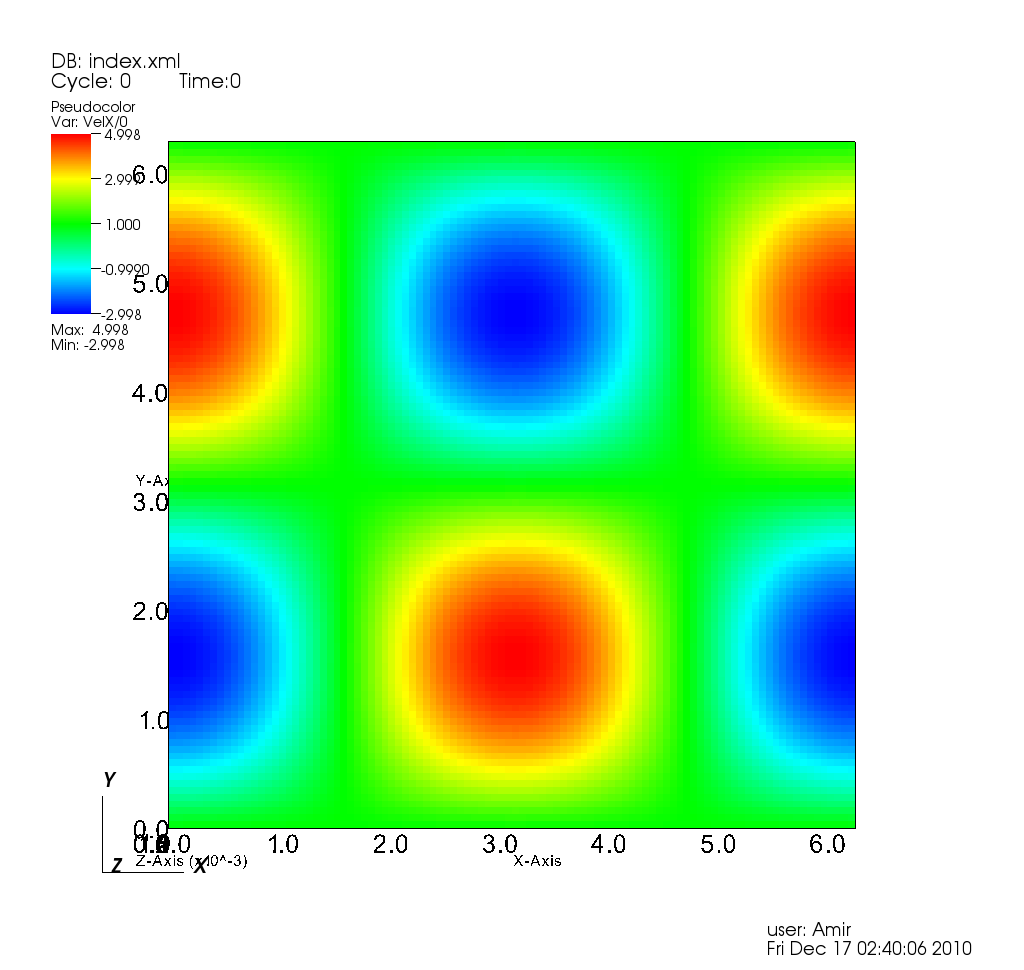
\includegraphics[width=2.27in]{t_0.png}
  \label{fig:vxt1}
  }
  \hfill
  \subfigure[]{
  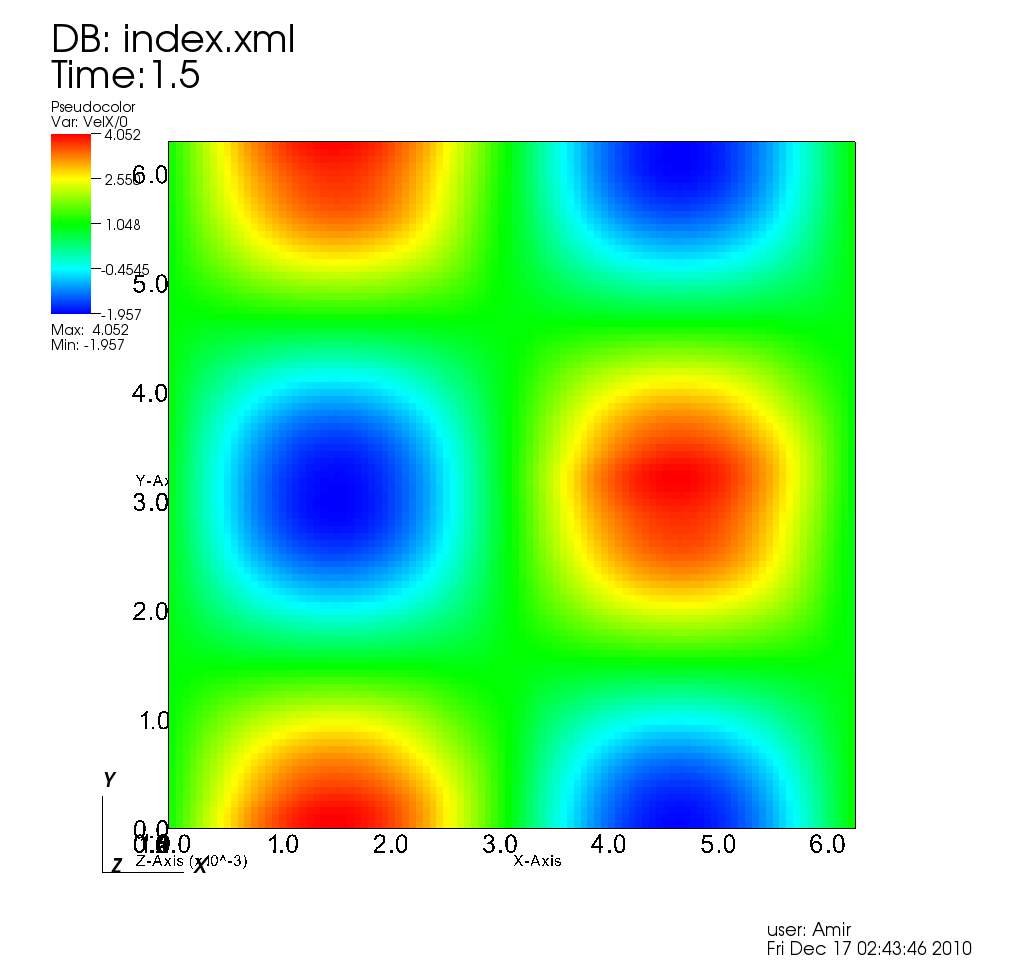
\includegraphics[width=2.27in]{t_1_5.png}
  \label{fig:vxt2}
  }
  \hfill
  \subfigure[]{
  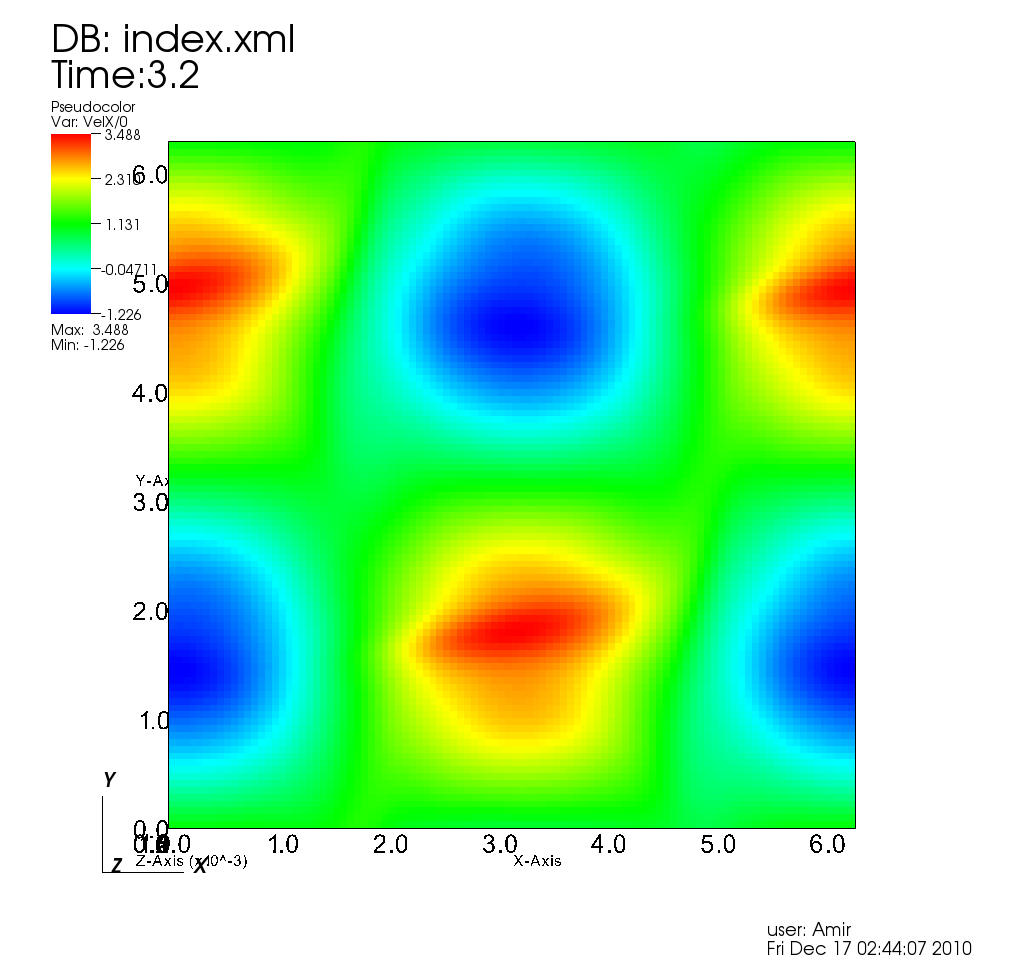
\includegraphics[width=2.27in]{t_3_2.png}
  \label{fig:vxt3}
  }
  \hfill
  \subfigure[]{
  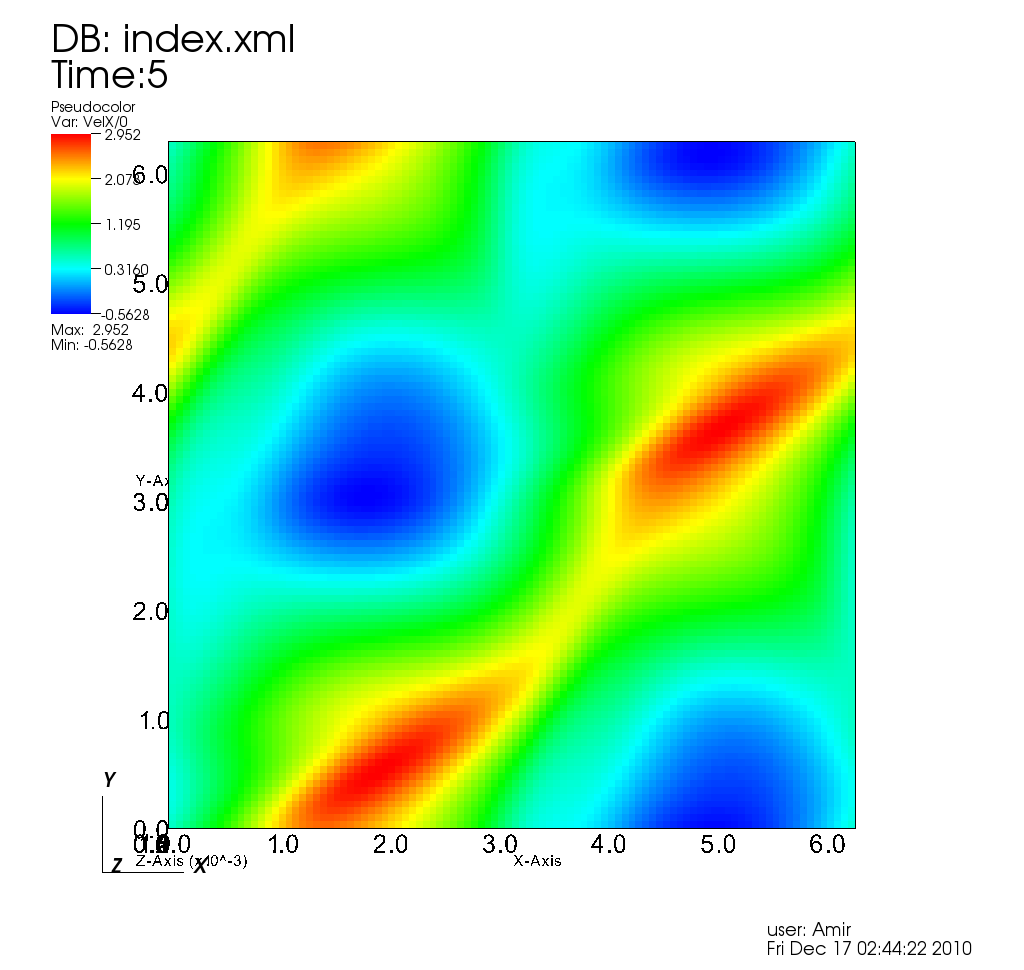
\includegraphics[width=2.27in]{t_5.png}
  \label{fig:vxt4}
  }
  \hfill
  \caption{\label{fig:velx} Pseudocolor profiles of velocity in $x$ direction at different snapshots of time \subref{fig:vxt1} t=0.0 s \subref{fig:vxt2} t=1.5 s \subref{fig:vxt3} t=3.2 s \subref{fig:vxt4} t=5.0 s} 
\end{figure*}

As you can see, if we go forward in time our solution for velocity in x direction will be unstable and in longer times the profile looks like a turbulent flow which is not right for Taylor Vortex flow. As we said this can be because of inconsistency between our solution and pressure analytical solution that we use from the beginning. 

\section{How to Do The Convergence Studies}

In this work we have done two kinds of convergence studies, grid convergence study and temporal convergence study. We know that our spatial accuracy is second order and our temporal accuracy is first order accurate. So, we are going to check the validity of these two.

In order to do the grid convergence study we looked at the four different grid resolutions for our domain, 50X50, 100X100, 200X200 and 400X400, and we chose 0.001, 0.0005, 0.00025 and 0.000125 respectively for their time step. However, we just looked at the results after the first time step. This is in  order to neglecting the temporal accuracy in the explicit solvers. Because, those terms will be calculated in the previous time step, therefore, in all of our cases they will be calculated at time zero. So, because of using the same time for these terms we don't let the time accuracy to influence our results for grid convergence study. 

Note that we have defined the variables that we want to study, in the input file in order to be saved, like VelX, VelY, XXVOL etc.

After running each case we need to follow these tasks in order to save the outputs in an appropriate way:

\begin{itemize}
\item
At first we have to extract the variables that we have defined in the input file. For doing this we use $lineextract$ method which is already in\\``uintah/build/StandAlone/tools/extractors''. Here you can see one example of using this method inorder to extract variables after running 50X50 case:

./lineextract -v VelY\_rhs -timestep 1 -istart 0 0 0 -iend 50 50 0 -uda ../../wasatch\_test.uda

Here you should put the name of the variable that you are looking for after the -v, after -timestep you specify your timestep and after -istart and iend you need to put the starting point of the domain that you are looking for and the end point. Here we just want to look at a plane because it is a two dimensional problem. After -uda you have to specify the address of your output ``.uda" file. You can also write only ``./lineextract" to see the help for this method.
\item
When you do the lineextract, the results will be appear in four long columns.The first three of them are just the node indices. So, in order to store them in a more applicable way at first we copy and paste this long column in a text file and we name it ``a.txt", then we use following lines of codes in MATLAB for example for the velocity in $y$ direction (VelY):

load a.txt\\
for i=1:50\\
b(:,i)=a((a(:,2)==i-1),4);\\
end\\
VelY50=b';\\
clear ans a i b

\item
We should do the same thing and extract velocity in $x$ direction. Also we need the location of x-staggered volumes and y staggered volumes which means (XXVOL, YXVOL, XYVOL, YYVOL).

\end{itemize}

We have to do all of this for all of the grid resolutions that we have and store the results somewhere with specific name to recognize. Then we can calculate the analytical velocities from the analytical solution that we have and look at the second norm of the difference between those velocities and our output velocities as the error.

Now if we plot the log of error vs the log of grid resolution ($\Delta$x) and compare it with the second and first order accurate results, we can see our grid convergence order os accuracy. Here you can see a sample code in MATLAB in this regard:\\
\\
t=0.001;\\
u=1-4*cos(XXVOL50-t).*sin(YXVOL50-t)*exp(-2*0.1*t);\\
err(1)=norm(u-VelX50);\\
t=0.0005;\\
u=1-4*cos(XXVOL100-t).*sin(YXVOL100-t)*exp(-2*0.1*t);\\
err(2)=norm(u-VelX100);\\
t=0.00025;\\
u=1-4*cos(XXVOL200-t).*sin(YXVOL200-t)*exp(-2*0.1*t);\\
err(3)=norm(u-VelX200);\\
t=0.000125;\\
u=1-4*cos(XXVOL400-t).*sin(YXVOL400-t)*exp(-2*0.1*t);\\
err(4)=norm(u-VelX400);\\
dx=[2*pi/50,2*pi/100,2*pi/200,2*pi/400];\\
O1=[err(1),err(1)/2,err(1)/4,err(1)/8];\\
O2=[err(1),err(1)/4,err(1)/16,err(1)/64];\\
plot(log(dx),log(err),'.r');\\
hold\\
plot(log(dx),log(O1),'.b');\\
plot(log(dx),log(O2),'.g');\\

For doing temporal convergence study you can follow the same tasks with small differences. Here we have to consider a specific point in time in order to look at and compare the errors in that time. In this work we chose 0.1 second as our reference point in time. So, we should extract for the appropriate time step in each case. 

At the end instead of the log of grid resolution we should plot with respect to the log of time step.

\section{Results From Convergence Studies} 
Here you can see the convergence studies results for velocity in $x$ and $y$ direction where we have compared our actual convergence with second and first accurate results.

\begin{figure*}[h]
\centering
  \hfill
  \subfigure[]{
  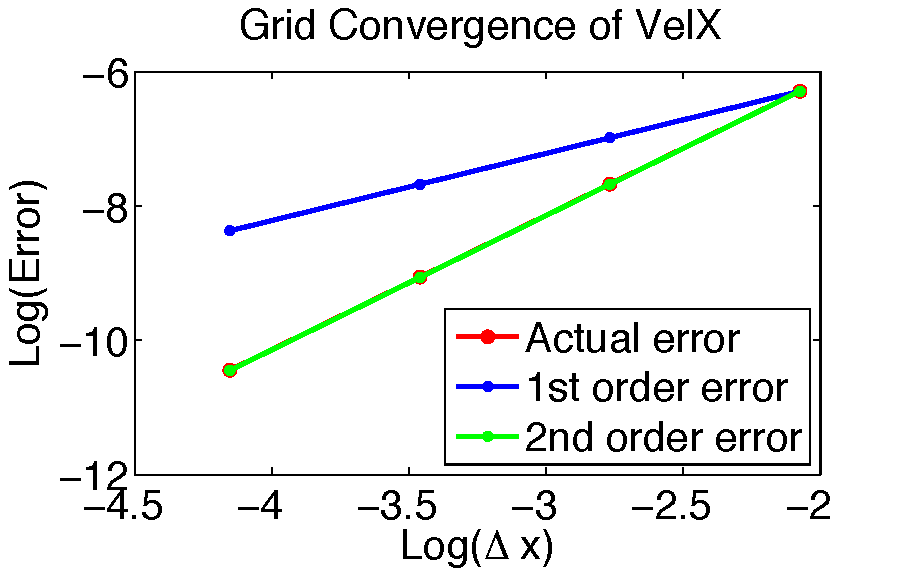
\includegraphics[width=2.27in]{grid_conv_velx_dx.pdf}
  \label{fig:vx_x}
  }
  \hfill
  \subfigure[]{
  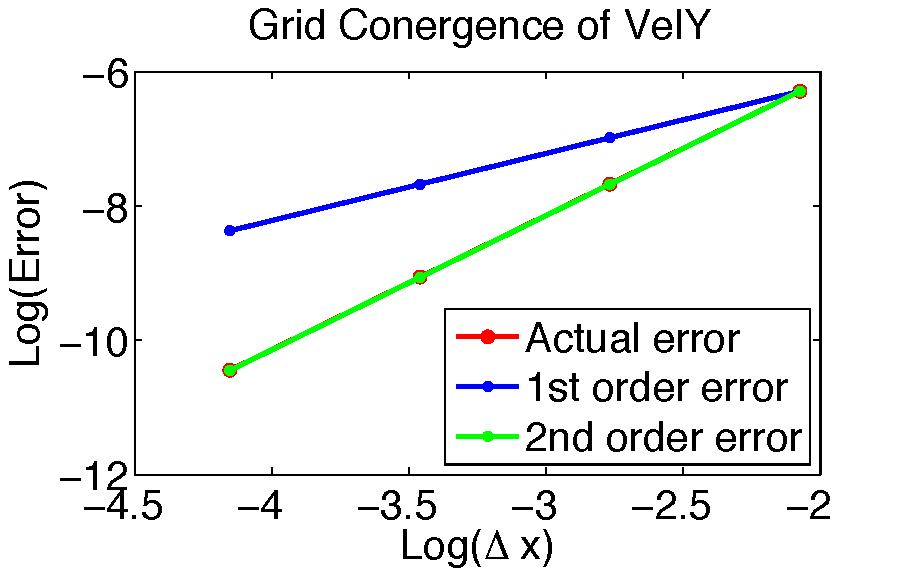
\includegraphics[width=2.27in]{grid_conv_vely_dx.pdf}
  \label{fig:vy_x}
  }
  \hfill
  \subfigure[]{
  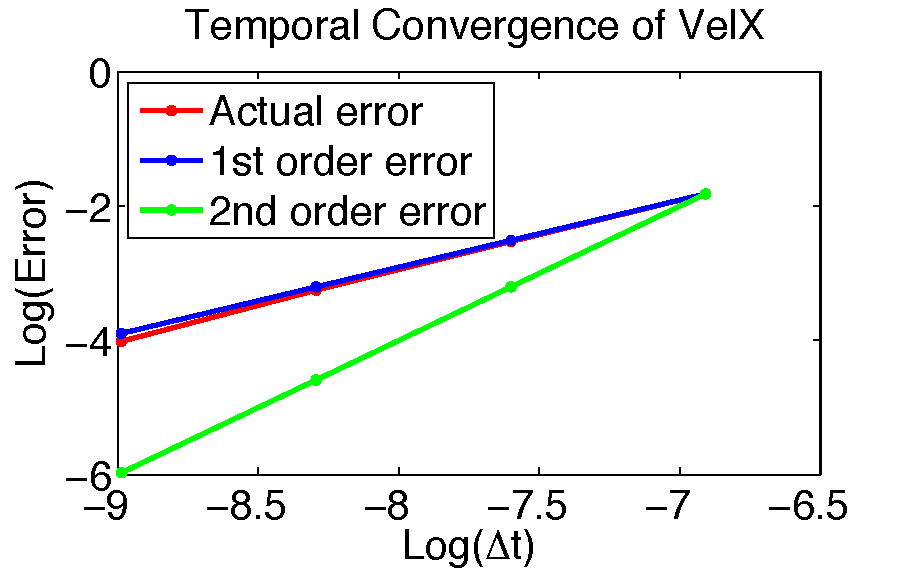
\includegraphics[width=2.27in]{grid_conv_velx_dt.pdf}
  \label{fig:vx_t}
  }
  \hfill
  \subfigure[]{
  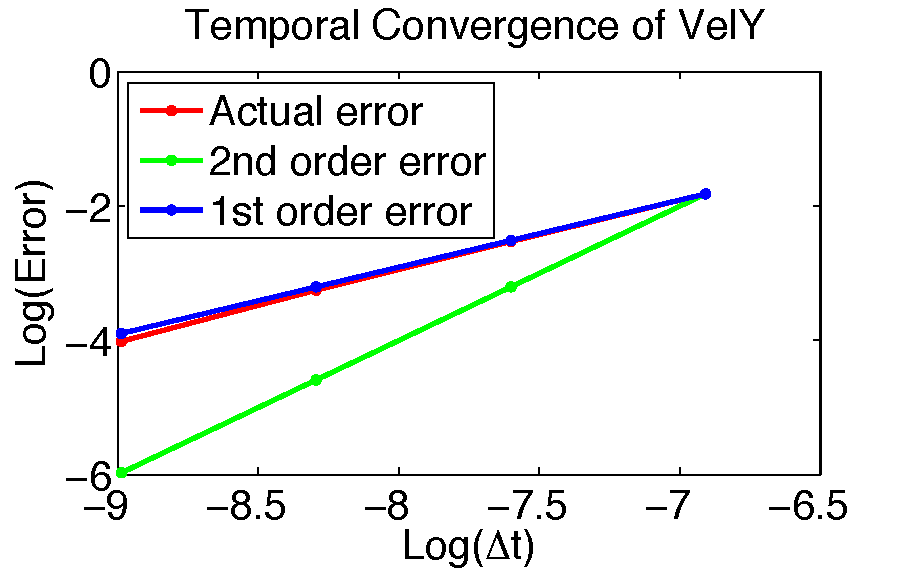
\includegraphics[width=2.27in]{grid_conv_vely_dt.pdf}
  \label{fig:vy_t}
  }
  \hfill
  \caption{\label{fig:conv} Convergence study of velocity in $x$ and $y$ directions \subref{fig:vx_x} Grid convergence of VelX \subref{fig:vy_x} Grid convergence of VelY \subref{fig:vx_t} Temporal convergence of VelX \subref{fig:vy_t} Temporal convergence of VelY} 
\end{figure*}

Here you can see that temporal convergence is first order accurate and grid convergence is second order accurate as we were expecting.
\clearpage
\bibliographystyle{unsrt}
\bibliography{Wasatch_MMS}

 \end{document}